%%%%%%%%%%%%%%%%%%%%%%%%%%%%%%%%%%%%%%%%%%%%%%%%%%%%%%%%%%%%%%%%%%%%%%%%%%%%%%%%
%                                                                              %
%   HIGZ  User Guide -- LaTeX Source                                           %
%                                                                              %
%   Chapter: Introduction to the HIGZ system                                   %
%                                                                              %
%   This document needs the following external EPS files:                      %
%     higzfig1.eps                                                             %
%                                                                              %
%   Editor: Michel Goossens / AS-MI                                            %
%   Last Mod.: 9 July 1993 oc                                                  %
%                                                                              %
%%%%%%%%%%%%%%%%%%%%%%%%%%%%%%%%%%%%%%%%%%%%%%%%%%%%%%%%%%%%%%%%%%%%%%%%%%%%%%%%
\Filename{H1HIGZIntroduction}
\chapter{Introduction}
The present document describes the \HIGZ~package
(High level Interface to Graphics and \ZEBRA). The package is a part of
larger system \PAW~(Physics Analysis Workstation)\cite{bib-PAW},
and it was originally implemented in order to provide a
graphics interface to \PAW. However \HIGZ~can also be used independently.
\par 
Graphics packages like \GKS~\cite{bib-GKS1} mediate the transition from user
programs (applications) to devices in a standardized way. The European effort 
to restrict High Energy Physics users to using only one such package (at least
for the 2D graphics), \GKS, will yield portability of application programs
between systems on which \GKS~is installed, and will make the application 
programs largely device-independent.
\par
These packages, however, have limitations. They do not foresee an acceptable way
of recording large volumes of graphical information in compact form with a 
convenient access method, for later manipulation. The \GKS~metafile is
\index{metafile} conceived as a vehicle to communicate series of pictures
between computers, but not for their subsequent manipulation. Also, the 
acceptance of \GKS, in particular by Laboratories outside Europe, is still
rather modest, and thus it is not a standard that the High Energy Physics
community can restrict itself to exclusively. We believe that the following
requirements must be met by the graphical output of \PAW:
\begin{enumerate}
\item The \PAW~picture data base must be fully transportable.
      \index{picture!data base}
\item It must have easily accessible units (pictures) for later manipulation.
\item The picture data base must be as compact as possible, and accessible in
      direct access mode.
\item The picture data base must be independent from the \UGP~and, a fortiori,
      from different implementations of the same graphics package.
\end{enumerate}
\par 
These requirements are not restricted to \PAW. They are common to many 
applications existing or under development. We therefore define below an 
interface package called \HIGZ, written in the context of \PAW, and aiming at
graphics applications of any nature, provided the level of functionality is 
similar. This package is basically a
thin layer between the user program (application) and an \UGP, offering the
following advantages:
\begin{enumerate}
\item An interface to a standard memory management system (\ZEBRA)
      \cite{bib-ZEBRA}, and through it a mechanism to store graphics data in a
      way which makes their organization and subsequent editing possible and 
      easy. The picture data base is also highly condensed and fully
      transportable. A picture editor is part of the package. It allows merging
      of pictures, editing of basic graphics primitives, operations onto 
      \HIGZ~structures, etc.
\item A \GKS~like user interface to the graphics package, keeping the program
      independent of the \UGP~installed.
\end{enumerate}
The level of \HIGZ~was deliberately chosen to be close to \GKS~and as basic as
possible. This makes the interface to \GKS~a very simple one, and preserves
full compatibility with the most important \UGPs. \HIGZ~does not introduce new
basic graphics features, and does not duplicate \GKS~functions. On the other
hand, some graphic macroprimitives are implemented, providing very frequently
used functions, such as graphs, circles and axis. The user will also be able to
call \GKS~directly in parallel with the use of \HIGZ.
 
Many of the underlying \GKS~concepts used by \HIGZ, e.g. the concepts of 
workstations and viewports, are well explained in \cite{bib-GKS1} and in
\cite{bib-GKS2}.
 
\HIGZ~is presently interfaced to several versions of \GKS. The version of 
\GKS~can be selected at compilation time by \PATCHY~control statements. On the
CERN central computers the \GKSGRAL~version is implemented. The list of the
different \GKS~versions, and of the values of \GKS~version-dependent 
parameters are specified in the appendix.
 
\HIGZ~is also interfaced the most important graphics packages such as \PHIGS,
\DI3000, \GDDM~(IBM), \GPR~(APOLLO), \GL~(Silicon Graphics).
Simple interfaces to the Tektronix/FALCO terminal and to the \XW~on
all the modern workstations are also available.
 
Thoughout this manual the graphics package on top of which \HIGZ~is installed is
referenced as ``\UGP''. When \HIGZ~has initialized the \UGP, the application 
program can call it directly. For example, if the \UGP~is \GKS, the application
program can access the segmentation facilities, but this will be not seen by 
\HIGZ. For all the additional functionalities provided by the \UGP, \HIGZ~is
transparent.
 
The \XW~interface is now one of the most frequently used on workstations
but also on mainframes like VAXes or IBM/VM machines. It has the advantages
of a great portability, good performances, and the possibility to be used
remotely through a network. The \HIGZ~interfaces to the \XW~is a small
layer callable by \FORTRAN~providing a convenient way to access the basic 
\XLIB~facilities from \FORTRAN. This interface is described in the chapter:
{\bf The \XW~interface routines}.
 
Most modern \UGP s usable from \HIGZ{} provide \PS~drivers. These drivers
can be used through \HIGZ, but a good uniform interface to \PS~is so important
that \HIGZ~has its own native \PS~driver independent from the \UGP~used
(see section \ref{IGMETA}).
 
In order to produce similar outputs even with different \UGP s, \HIGZ~has its own
line styles, hatches, marker types and text independent from the \UGP. 
Thus it is possible to use all the basic tools even on a very simple terminal (for
example a FALCO).
 
\index{picture!data base}
\Filename{H2Functionality}
\section{Functionality}
The \HIGZ~system is subdivided into three main sets of functions:
\begin{enumerate}
\item Basic graphics functions ({\tt I...} routines), interfacing to the \UGP,
      with calling sequences identical to those of \GKS.
\item Higher-level macroprimitives ({\tt IG...} routines), and the related 
      control routines.
\item Memory management function ({\tt IZ...} routines), interfacing to the
      memory management system (\ZEBRA).
\end{enumerate}
 
The {\tt IG...} and the {\tt I...} functions act on the screen and/or on the
data structure in main storage. All graphics functions producing a graphics
object are able to direct the output:
\begin{itemize}
\item to the display device
\item to the data management system
\item to both
\end{itemize}
 
These actions are controlled by a switch set by the routine \Rind{IGZSET}.
 
The {\tt IZ...} functions are the memory management functions. They act on the
data structure in main storage and on the data stored on disk.
This is particularly useful during an interactive session, as the user is 
able to ``replay'' pictures previously created, with no need to recall the
application program, but just accessing the picture data base.
 
These two sets of functions are described pictorially on the figure 
\ref{HIGZSYS}.
 
\begin{Fighere}
\begin{center}\mbox{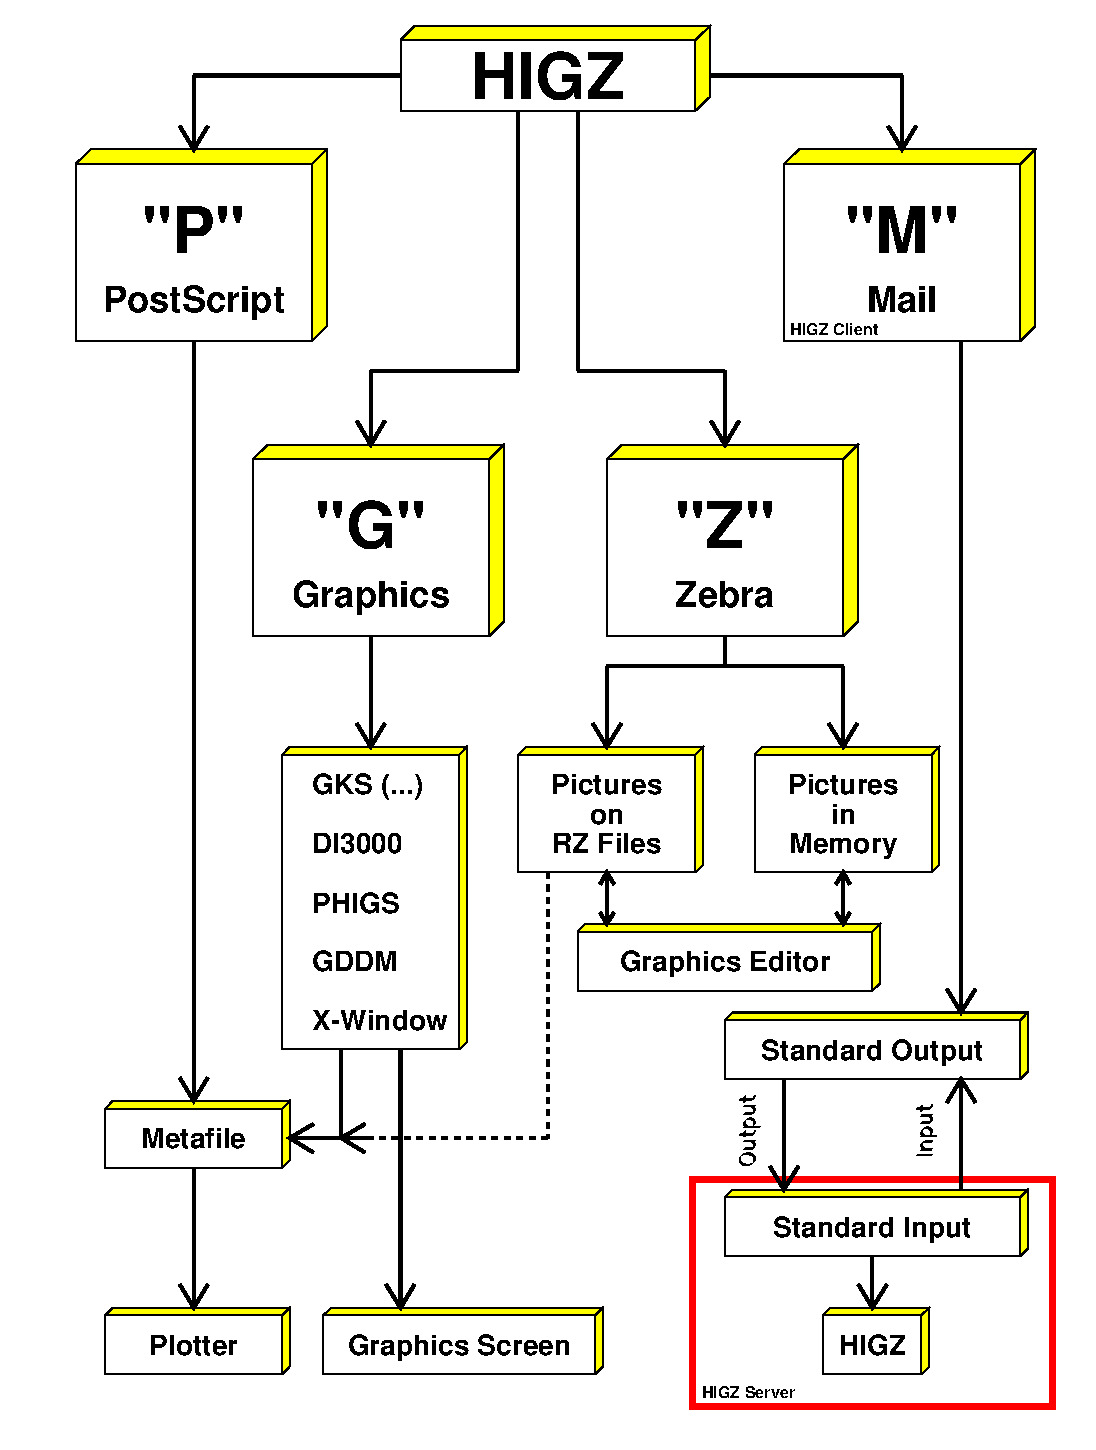
\epsfig{file=higzsys.eps,height=15cm}}\end{center}
\caption{Structure of the \HIGZ~system.}
\label{HIGZSYS}
\end{Fighere}
 

